\documentclass[11pt, a4paper]{article}

\usepackage[utf8]{inputenc}
\usepackage[italian]{babel}
\usepackage[T1]{fontenc}
\usepackage{geometry}
\usepackage{amsmath}
\usepackage{amssymb}
\usepackage{graphicx}
\usepackage{subcaption}
\usepackage{hyperref}
\usepackage{booktabs}
\usepackage{listings}
\usepackage[most]{tcolorbox}
\usepackage{xcolor}

\geometry{a4paper, margin=2.3cm}

\lstset{
    backgroundcolor=\color{gray!5},
    basicstyle=\ttfamily\small,
    breaklines=true,
    keywordstyle=\color{blue!80!black}\bfseries,
    commentstyle=\color{green!50!black}\itshape,
    stringstyle=\color{orange},
    frame=single,
    rulecolor=\color{gray!30},
    numbers=none,
    showstringspaces=false
}

\title{
    \textbf{Relazione del Progetto di Programmazione per la Fisica} \\
    \vspace{0.3cm}
    \large Simulazione dinamica ed emergenza collettiva del comportamento di stormi nel modello dei Boids con SFML
}
\author{Borchetta Simone, Genovesi Antonio}
\date{28 agosto 2026}

\begin{document}
\maketitle
\hrule
\vspace{0.5cm}
\section*{Modifiche dalla consegna precedente}
Rispetto alla consegna del 15 luglio 2026 il progetto è stato sottoposto a modifiche e revisioni. Riportiamo di seguito i cambiamenti salienti:
\begin{itemize}
    \item \textbf{Unificazione del namespace: }Nella stesura precedente, per evitare conflitti di nomi, il codice era stato ripartito in diversi namespace indipendenti 
    (\texttt{phy}, \texttt{boids}, \texttt{stats}, \texttt{sim}). Per rispettare rigorosamente le specifiche del progetto, tutte le entità del programma (tipi, funzioni, classi) sono state ora migrate e dichiarate all'interno di un unico namespace (\texttt{bs}) dedicato alla simulazione
    \item \textbf{Strumento di Formattazione: }Come richiesto dalle linee guida, il file di configurazione \texttt{.clang-format} utilizzato per definire le regole stilistiche del codice è stato esplicitamente incluso nell'archivio di consegna, insieme al file \texttt{CMakeLists.txt} e alle altre dipendenze.  
    \item \textbf{Ottimizzazione delle dichiarazioni e delle definizioni delle Funzioni (Parametri e Return Types): }È stata condotta una revisione sistematica delle interfacce delle funzioni. Si è prestata particolare attenzione al passaggio appropriato dei parametri, implementando il passaggio per const reference (\texttt{const T\&}) 
    per gli oggetti complessi (es. le strutture dati della configurazione o vettori di grandi dimensioni) e mantenendo il passaggio per valore (by value) per i tipi primitivi. Parallelamente, sono stati ottimizzati i return types per prevenire copie non necessarie.
    \item \textbf{Uso di this e rimozione di self\_index, cambiamento dei return type di \texttt{Boid::update}: }Sono stati implementati dei range-for loop nelle funzioni di aggiornamento della simulazione. Dopo aver tentato di far riconoscere al boid se stesso mediante un approccio geometrico non sempre efficace (controllando che la distanza tra i due boid fosse pari a 0), abbiamo deciso di modificare i metodi della classe \texttt{Boid} ad esempio: \texttt{Boid::compute\_cohesion}, \texttt{Boid::compute\_alignment}, \texttt{Boid::compute\_separation}... in modo da riconoscere il boid attraverso gli indirizzi di memoria.
    A tal proposito abbiamo dovuto modificare interamente la logica di programmazione, dal momento che inizialmente si confrontavano \texttt{boids} appartenenti a due flock diversi (\texttt{flock}, \texttt{next\_flock}). Come conseguenza è variato il codice inerente al metodo \texttt{Boid::update} che restituisce una copia modificata che viene, in seguito all'applicazione di forze attraverso \texttt{Boid::apply\_force}, inserita in \texttt{next\_flock}. 
    \item \textbf{Uso appropriato di static: }Abbiamo eliminato l'utilizzo di \texttt{static} nel codice.
    \item \textbf{Uso di \texttt{std::sqrt}: }Rispetto alla precente versione del progetto è stato limitato l'utilizzo della funzione \texttt{std::sqrt} della Standard Library. Abbiamo convertito diversi controlli limitandoli a confronti tra quadrati delle variabili. In questo modo è stato realizzato un codice più leggero e ottimizzato rispetto alle versioni precedenti.
    \item \textbf{Modifiche relative alla relazione: }Dati i cambiamenti del codice abbiamo provveduto a perfezionare la descrizione di quest'ultimo nella relazione da consegnare. Abbiamo inoltre aggiunto nuove spiegazioni in quest'ultima relative alle configurazioni iniziali della simulazione. Sono stati documentati a fondo relazione i risultati ottenuti mediante l'utilizzo di immagini.

\end{itemize}
\section*{Riassunto}
Il progetto implementa una simulazione numerica del modello dei \textit{Boids}, introdotto da Craig Reynolds nel 1986 per descrivere il comportamento collettivo e coordinato (\textit{flocking}) di stormi di uccelli o banchi di pesci. Ogni agente evolve nel tempo seguendo semplici regole locali geometriche e cinematiche. La simulazione è interamente realizzata in C++ ed integra la libreria grafica SFML per la visualizzazione bidimensionale in tempo reale, una componente statistica per l'analisi dei dati in esecuzione e un modulo interattivo che prevede la presenza di agenti predatori (\textit{hunters}) e forze esterne pilotabili dall'utente tramite mouse.

\section{Introduzione e Tema del Progetto}
\label{sec:introduzione}
Il presente lavoro implementa uno dei temi d'esame del corso. L'obiettivo principale è studiare simulazione delle proprietà emergenti di un sistema complesso auto-organizzato, basato sul modello di \textit{flocking} dei Boids.

All'inizio della simulazione, le posizioni e le velocità dei boids sono del tutto casuali e disordinate. Tuttavia, le interazioni a corto raggio tra i vicini fanno in modo che si formi uno stormo unito e coerente. Il funzionamento del modello si basa sul concetto di \textit{proprietà emergente}: non esiste un leader che coordina il movimento, ma ogni agente decide come muoversi guardando solo gli altri boids che si trovano all'interno del suo raggio visivo ($d$). Ad ogni passo temporale $\Delta t$, il ciclo di esecuzione prevede che ogni boid scansioni l'ambiente circostante, identifichi i propri vicini e calcoli vettorialmente le forze d'interazione. La somma di questi contributi determina la nuova velocità e, di conseguenza, la posizione successiva dell'agente sullo schermo.

\section{Modello Fisico e Regole di Volo}
\label{sec:modellofisico}
Le regole di volo servono a calcolare le variazioni di velocità da applicare a ciascun boid. Matematicamente, l'aggiornamento della velocità $\vec{v}_{b_i}$ e della posizione $\vec{x}_{b_i}$ di ogni boid $b_i$ avviene tramite le seguenti equazioni:
\begin{align}
    \vec{v}_{b_i} &= \vec{v}_{b_i} + \vec{v}_1 + \vec{v}_2 + \vec{v}_3 \\
    \vec{x}_{b_i} &= \vec{x}_{b_i} + \vec{v}_{b_i} \Delta t
\end{align}
I vettori $\vec{v}_1$, $\vec{v}_2$ e $\vec{v}_3$ sono i contributi calcolati applicando le tre regole di Reynolds sui boids vicini. Dato il raggio visivo $d$, l'insieme dei vicini $N_i$ del boid $i$-esimo contiene tutti gli agenti che si trovano a una distanza minore di $d$:
\begin{equation}
    N_i = \{ b_j \;\vert\; 0 < \lVert \vec{x}_i - \vec{x}_j \rVert < d \}
\end{equation}

\subsection{Le Regole Classiche di Reynolds}
Il comportamento complessivo dello stormo emerge dalla combinazione lineare di tre forze fondamentali:
\begin{itemize}
    \item \textbf{Separazione:} Ha lo scopo di evitare che i boids collidano tra loro. L'accelerazione repulsiva si attiva solo se la distanza mutua è inferiore a un raggio critico di sicurezza $d_s < d$:
    \begin{equation}
        \vec{v}_1 = -s \sum_{j \neq i} (\vec{x}_{b_j} - \vec{x}_{b_i}) \quad \text{se } \lVert \vec{x}_{b_i} - \vec{x}_{b_j} \rVert < d_s
    \end{equation}
    L'uso della distanza come fattore cinematico garantisce un puntamento e un allontanamento graduale, la cui intensità è regolata dal coefficiente $s$.
    
    \item \textbf{Allineamento:} Fa in modo che gli agenti tendano a procedere nella stessa direzione dello stormo, sincronizzando i vettori di velocità relativi:
    \begin{equation}
        \vec{v}_2 = a \left( \frac{1}{n-1} \sum_{j \neq i} \vec{v}_{b_j} - \vec{v}_{b_i} \right)
    \end{equation}
    Il contributo si ottiene sottraendo la velocità attuale del boid $b_i$ dalla media delle velocità dei suoi vicini, pesata per un fattore $a < 1$ che determina la rapidità di sterzata.
    
    \item \textbf{Coesione:} Induce l'agente a volare verso il baricentro locale dei boids circostanti per mantenere l'unità dello stormo. Il centro di massa $\vec{x}_c$ è calcolato come:
    \begin{equation}
        \vec{x}_c = \frac{1}{n-1} \sum_{j \neq i} \vec{x}_{b_j}
    \end{equation}
    La componente di velocità $\vec{v}_3$ si ricava di conseguenza come attrazione verso tale baricentro tramite un coefficiente di accoppiamento $c$:
    \begin{equation}
        \vec{v}_3 = c (\vec{x}_c - \vec{x}_{b_i})
    \end{equation}
\end{itemize}

\subsection{Modellizzazione della Predazione: gli \textit{Hunters}}
Per inserire un elemento di disturbo nello stormo, il programma prevede la presenza dei cacciatori (\textit{hunters}). Rispetto ai boids ordinari, gli \textit{hunters} hanno parametri diversi: possiedono dimensioni geometriche maggiori e una velocità massima più elevata.

Il loro diverso comportamento segue dall'applicazione di forze centrali attraveso la funzione \texttt{apply\_force}:
\begin{itemize}
    \item \textbf{Separazione tra i Cacciatori:} Gli \textit{hunters} non si muovono in modo del tutto isolato; per evitare di andarsi a sbattere addosso a vicenda, la regola della separazione rimane attiva all'interno del loro gruppo.
    \item \textbf{Propulsione:} Ciascun cacciatore viene spinto costantemente nella direzione in cui si sta già muovendo. Il programma calcola una forza diretta verso un punto proiettato in avanti nel tempo lungo la sua traiettoria ($\vec{x}_{\text{hunter}} + 4\vec{v}_{\text{hunter}}$) al fine di rendere più fluida la simulazione.
    \item \textbf{Attrazione verso il Centro dello Stormo:} Contemporaneamente, il cacciatore viene attratto dal centro di massa dello stormo dei boids ($\vec{x}_c$). Questa forza centrale serve a fargli inseguire il gruppo, e la sua intensità viene dimezzata (moltiplicata per $-0.5$) rispetto al parametro standard.
\end{itemize}

Non appena un \textit{hunter} entra nel raggio di percezione dei boid (\texttt{influence\_radius}), i boids vengono spinti da una forza repulsiva che si somma vettorialmente alle altre forze dello stormo ma, data la sua intensità, domina la deviazione della traiettoria spingendoli nella direzione opposta.

\section{Scelte Progettuali e Ripartizione del Codice}
\label{sec:progettazione}
Il codice è scritto in C++ su diversi file:

\begin{itemize}
    \item \textbf{\texttt{vector2d.hpp}}: Contiene le definizioni dell'interfaccia per la struttura dati \texttt{Vector2D}, progettata per la gestione di vettori nello spazio bidimensionale $\mathbb{R}^2$.
    \item \textbf{\texttt{vector2d.cpp}}: Contiene le definizioni delle funzioni della struttura dati dichiarata nell'header \texttt{vector2d.hpp}. Inoltre sono presenti gli overload degli operatori dichiarati in esso.
    \item \textbf{\texttt{boid.hpp}}: Definisce la classe \texttt{Boid}, che costituisce l'agente fondamentale della simulazione. Questa classe incapsula lo stato fisico dell'entità (posizione e velocità) e i metodi necessari per implementare il comportamento collettivo basato sul modello di Reynolds (separazione, allineamento e coesione).
    \item \textbf{\texttt{boid.cpp}}: Implementa la logica comportamentale e cinetica della classe \texttt{Boid}. Basandosi sul modello di Reynolds, il codice traduce le interazioni locali tra le entità in vettori di forza, determinando il movimento fluido e collettivo tipico di uno stormo.
    \item \textbf{\texttt{statistics.hpp}}: Contiene le dichiarazioni dell'interfaccia per il modulo di analisi statistica, progettato per elaborare i dati relativi a un gruppo di oggetti di tipo \texttt{Boid} (tipicamente rappresentanti una simulazione di stormo).
    \item \textbf{\texttt{statistics.cpp}}: Fornisce l'implementazione logica delle funzioni di analisi statistica per lo stormo di Boid. Utilizza algoritmi della libreria standard C++ (\texttt{<algorithm>}, \texttt{<numeric>}) per elaborare in modo efficiente le proprietà del vettore flock.
    \item \textbf{\texttt{simconfig.hpp}}: Definisce la struttura dati \texttt{SimConfig}, che centralizza tutti i parametri di configurazione necessari al motore di simulazione. Tale approccio permette di separare la logica dei parametri dai componenti dinamici (i \textit{Boid}), facilitando la gestione delle impostazioni sia globali che specifiche per eventuali sottogruppi (es. predatori o \textit{kettle}). Abbiamo implementato questo \textit{header file}, incluso ad esempio in \texttt{boid.cpp} e in \texttt{boid.hpp}, in modo da poter dichiarare e definire delle funzioni che accettassero in input una singola struct, al posto di svariati parametri. Sono state dichiarate delle funzioni necessarie alla configurazione della simulazione, qualora si volessero utilizzare dei parametri da passare attraverso \texttt{std::cin}.
    \item \textbf{\texttt{simconfig.cpp}}: Implementa la logica di inizializzazione e configurazione dinamica dei parametri di simulazione. Gestisce l'interazione con l'utente tramite standard input per definire le caratteristiche dello stormo e dei predatori (\textit{hunter}), includendo meccanismi di validazione dei dati in ingresso. 
    \item \textbf{\texttt{simulation.hpp}}: Contiene le dichiarazioni dell'interfaccia per il modulo di aggiornamento fisico della simulazione. In esso è presente la dichiarazione della funzione \texttt{update\_physics}, che gestisce l'evoluzione temporale dello stormo (\textit{flock}) e di eventuali sotto-gruppi (\textit{kettle}), applicando le regole di comportamento (\textit{flocking}) basate sulle configurazioni (\texttt{SimConfig}) e sugli input dell'utente (posizione del mouse e stati dei tasti). Inoltre, è presente la funzione \texttt{entity\_gen} per la generazione dello stormo, meglio descritta di seguito.
    \item \textbf{\texttt{simulation.cpp}}: Implementa la logica di aggiornamento temporale della simulazione 
    \newline (\texttt{update\_physics}). Esso funge da motore principale, coordinando il calcolo delle forze, l'applicazione delle regole di comportamento (\textit{flocking}) e la gestione dei vincoli spaziali per le entità (\textit{Boid}) presenti sia nello stormo principale che nel sotto-gruppo dei predatori (\textit{kettle}).
    \item \textbf{\texttt{render.hpp}}: Viene dichiarata l'interfaccia per il modulo di visualizzazione grafica, che utilizza la libreria SFML (\textit{Simple and Fast Multimedia Library}) per l'interfacciamento con l'hardware grafico. Il modulo si occupa della traduzione dello stato logico della simulazione (vettori di entità e dati statistici) in rappresentazioni visive su finestra.
    \item \textbf{\texttt{render.cpp}}: Contiene l'implementazione del motore grafico del progetto, che traduce lo stato numerico della simulazione (posizioni, velocità e dati statistici) in un output visivo mediante la libreria \textit{SFML}. Il modulo segue un pattern di rendering immediato, ottimizzato per l'aggiornamento costante durante il ciclo di gioco (\textit{game loop}).
\end{itemize}
Nell'archivio inviato sono presenti file come \texttt{CMakeLists.txt}, \texttt{.clang-format}, \texttt{doctest.h}, \newline \texttt{arial.ttf} utilizati nello sviluppo del progetto.
\subsection{Scelte Algoritmiche e Dinamica delle Forze}
\subsubsection{Configurazione Iniziale e Parametri di Input}
Per garantire flessibilità nell'analisi della simulazione, la funzione \texttt{get\_user\_config()} richiede all'avvio alcuni parametri di input da terminale standard. L'utente può scegliere tra due modalità principali di inizializzazione:
\begin{itemize}
    \item \textbf{Configurazione Predefinita:} Avvia immediatamente la simulazione caricando un set di parametri fisici standard (velocità massime, coefficienti delle tre regole e raggi di influenza) pre-impostati per garantire uno stormo stabile e visivamente coerente.
    \item \textbf{Configurazione Personalizzata:} Consente all'utente di modificare manualmente i singoli coefficienti per studiare comportamenti alternativi e fluttuazioni del sistema.
\end{itemize}
Per agevolare le procedure di configurazione della simulazione ed evitare l'inserimento manuale interattivo a ogni avvio, l'acquisizione dei parametri tramite \texttt{std::cin} è stata progettata per supportare la redirezione dell'input da un file di testo. È sufficiente creare un file (ad esempio quello da noi consegnato nell'archivio \texttt{configuration.txt}) contenente i valori disposti sequenzialmente, separati da ritorni a capo, nello stesso ordine in cui vengono richiesti dal prompt del programma.

A titolo di esempio, il contenuto del file per una configurazione personalizzata con 600 boids e 2 predatori si presenta in questo modo:
\begin{tcolorbox}[
  colback=gray!5!white,
  colframe=gray!75!black,
  title=Esempio di \texttt{configuration.txt} commentato,
  arc=1mm
]
\small\ttfamily
\begin{tabular}{ll}
n       & \textcolor{gray}{\% Impostazione configurazione personalizzata} \\
        & \textcolor{gray}{\% (Riga vuota)} \\
600     & \textcolor{gray}{\% Numero di boids} \\
60      & \textcolor{gray}{\% Visual range (d)} \\
20      & \textcolor{gray}{\% Separation radius (ds)} \\
0.8     & \textcolor{gray}{\% Separation factor (s)} \\
0.5     & \textcolor{gray}{\% Alignment factor (a)} \\
0.01    & \textcolor{gray}{\% Cohesion factor (c)} \\
        & \textcolor{gray}{\% (Riga vuota)} \\
2       & \textcolor{gray}{\% Numero di hunters}
\end{tabular}
\end{tcolorbox}
Indipendentemente dalla modalità scelta, il sistema richiede esplicitamente l'inserimento del \textbf{numero di cacciatori (\textit{hunters})}, anche nullo, da generare.
\paragraph{Esempio di esecuzione con configurazione personalizzata}
Di seguito si riporta un esempio di input interattivo consigliato per la valutazione del comportamento collettivo:
\begin{lstlisting}
Would you like to start the boid simulation with the default parameters? (y/n): n
Enter number of boids: 150
Enter the visual range (d): 60
Enter the separation radius (ds): 20
Enter the separation factor (s): 0.8
Enter the alignment factor (a): 0.5
Enter the cohesion factor (c): 0.01
Enter number of hunters: 3
\end{lstlisting}
\subsubsection{Generazione di flocks e kettles}
La generazione sia degli stormi di Boid (\textit{flocks}) che dei gruppi di predatori (\text{kettle}) è affidata alla funzione \texttt{entity\_gen}. La funzione riceve in input un oggetto di tipo \texttt{bs::SimConfig} contenente tutti i parametri necessari per configurare l'entità. La funzione esegue un controllo sugli input: per gli stormi di \textit{boids} viene richiesto un numero di entità strettamente positivo, mentre per gli \textit{hunters} un numero non negativo. In caso di parametri non validi, il sistema solleva un'eccezione \texttt{std::runtime\_error}.
Utilizzando il motore di numeri casuali \texttt{std::default\_random\_engine} la funzione distribuisce le entità nello spazio $\mathbb{R}^2$. Le coordinate ($x$, $y$) sono calcolate entro i bordi definiti dalla configurazione, applicando un margine di sicurezza. Ogni entità viene inizializzata con un vettore velocità ($v_x$,$v_y$) casuale e controlla il valore booleano \texttt{is\_hunter} presente nella configurazione: se esso ha valore \texttt{true}, vengono applicati i limiti di velocità specifici del predatore.


\subsubsection{Regole di volo}
Sono state implementate le regole di volo presentate in Sezione \ref{sec:modellofisico}:
\begin{itemize}
    \item \texttt{compute\_separation}: impedisce ai boids di sovrapporsi o scontrarsi. Per ogni vicino all'interno del \texttt{separation\_radius} calcola un vettore repulsivo che allontana il boid corrente. L'intensità della spinta è regolata attraverso il \texttt{separation\_factor}.
    \item \texttt{compute\_alignment}: permette allo stormo di muoversi in modo coordinato. Il boid calcola la media dei vettori velocità dei vicini entro il proprio \texttt{visual\_range} e genera una forza che tende ad allineare la propria direzione a quella del gruppo, pesata dall'\texttt{alignment\_factor}.
    \item \texttt{compute\_cohesion}: spinge il boid verso il centro di massa dei vicini percepiti, garantendo che lo stormo rimanga coeso e non si disperda, regolata dal \texttt{cohesion\_factor}.
\end{itemize}
Sono state costruite delle funzioni di supporto al movimento delle entities:
\begin{itemize}
    \item \texttt{limit\_velocity}: assicura che ogni boid rimanga entro un intervallo di velocità realistico (\texttt{min\_vel} e \texttt{max\_vel}), evitando accelerazioni infinite che renderebbero instabile la simulazione.
    \item \texttt{apply\_toroidal\_boundary}: crea uno spazio ciclico (se un boid esce a destra, rientra a sinistra).
    \item \texttt{apply\_window\_boundary}: genera una forza repulsiva verso l'interno quando il boid si avvicina ai bordi della finestra.
    \item \texttt{apply\_force}: permette di applicare influenze dirette, come l'attrazione/repulsione causata dal mouse o dai predatori, calcolando un vettore basato sulla distanza rispetto a un punto di influenza.
\end{itemize}

\subsubsection{Evoluzione temporale}
L'evoluzione temporale del sistema adotta un approccio di aggiornamento sincrono delle coordinate. All'interno della funzione \texttt{update\_physics}, lo stato dello stormo e del kettle al tempo $t$ viene letto per calcolare i contributi di forza su ciascun agente; le nuove posizioni e velocità al tempo $t+\Delta t$ vengono quindi generate e salvate nei vettori ausiliari \texttt{next\_flock} e \texttt{next\_kettle}. Successivamente, il riassegnamento dello stato avviene tramite \texttt{std::move(next\_flock)} e \texttt{std::move(next\_kettle)}. Questo approccio elimina asimmetrie temporali fittizie dovute all'ordine sequenziale dell'elaborazione nei cicli \texttt{for}.

L'evoluzione dinamica ad ogni passo di integrazione si articola nelle seguenti fasi:
\begin{enumerate}
    \item \textbf{Aggiornamento dei Boids:} Il metodo \texttt{update} della classe \texttt{Boid} calcola le componenti di accelerazione dovute alle tre regole di Reynolds (separazione, allineamento e coesione) calcolate rispetto agli altri componenti dello stormo. A queste si aggiunge la forza repulsiva generata da ciascun \textit{hunter} presente nel vettore \texttt{kettle}, simulando l'istinto di fuga dei boids. Vengono infine applicati i vincoli di bordo (toroidali o confinati) per mantenere le entità nell'area di simulazione.
    \item \textbf{Aggiornamento dei Hunters} Il codice gestisce una flotta di \textit{hunters} distinta (\texttt{kettle}), caratterizzata da limiti di velocità superiori. I cacciatori inseguono il centro di massa dei boids percepiti e mantengono una distanza di sicurezza tra loro tramite la sola regola di volo attiva: quella di separazione. Le forze integrate nel loro vettore velocità ne determinano lo spostamento finale.
    \item \textbf{Interattività Utente:} L'utente può perturbare il sistema in tempo reale tramite input asincroni del mouse. La pressione del tasto destro genera una forza attrattiva verso le coordinate del cursore, mentre il tasto sinistro applica una forza repulsiva.
\end{enumerate}

\subsubsection{Generazione dei grafici attraverso SFML}
Il modulo di rendering grafico è stato sviluppato, come anticipato, nel file \texttt{render.cpp}, che si basa sull'aggiornamento ciclico di primitive grafiche all'interno di una \texttt{sf::RenderWindow}. Il file si occupa di tre funzionalità principali:
\begin{enumerate}
    \item Rendering delle entità: le funzioni \texttt{render\_flock} e \texttt{render\_kettle} visualizzano gli stormi e i predatori attraverso oggetti di tipo \texttt{sf::ConvexShape}. Le forme vengono dichiarate come \texttt{static} con un flag \texttt{initialized}, che garantisce che la geometria venga definita una volta sola all'avvio, risparmiando risorse computazionali durante il \textit{game loop}. Per ogni entità il codice esegue due operazioni prima di richiamare \texttt{window.draw()}: vengono allineate la forma alle coordinate ($x$, $y$) del \texttt{boid} attraverso la funzione \texttt{set\_Position}. Attraverso la funzione \texttt{set\_Rotation} viene orientato il triangolo in base all'angolo del vettore velocità, permettendo all'utente di percepire la direzione del moto del \texttt{boid}.
    \item Rappresentazione dei dati: la funzione \texttt{render\_histogram} trasforma un insieme di dati statistici (bins di velocità) in un istogramma grafico. L'altezza di ogni barra viene calcolata proporzionalmente al valore massimo presente nel dataset (\texttt{max\_count}) rispetto all'altezza totale disponibile(\texttt{bounds.height}). Il ciclo \texttt{for} crea rettangoli (\texttt{sf::RectangleShape}) per ogni bin, posizionandoli orizzontalmente in modo equispaziato. Vengono utilizzate \texttt{sf::Text} per visualizzare i valori numerici e le etichette dell'asse X. Il font viene caricato una sola volta staticamente, evitando operazioni di I/O disco onerose a ogni fotogramma.
    \item Gestione degli Eventi: la funzione \texttt{handle\_events} funge da interfaccia di controllo tra l'utente e la simulazione. Si utilizza \texttt{window.pollEvent} per monitorare costantemente le azioni dell'utente, come la chiusura delle finestre. La pressione di tasti specifici modifica lo stato della simulazione in tempo reale: premendo il tasto 'B' si cambia la modalità dei confini (toroidal $\leftrightarrow$ bounded), premendo il tasto 'S' apre o chiude la finestra secondaria dedicata alle statistiche, gestendo dinamicamente il ciclo di vita della \texttt{statsWindow} (creazione e distruzione).
\end{enumerate}
\subsection{Strategia di Test e Verifica del Codice}
Per garantire l'affidabilità del simulatore e la correttezza delle equazioni fisiche implementate, si è adottato il framework di unit testing \texttt{doctest}. La suite automatizzata è suddivisa in tre macro-aree che validano le componenti critiche del sistema:

\begin{itemize}
    \item \textbf{Algebra vettoriale (\texttt{Vector2D}):} 
    I test verificano la rigorosa correttezza aritmetica degli overload degli operatori ($+$, $-$, $*$, $/$, ecc.). Oltre al calcolo della norma euclidea e della distanza, viene validata la funzione \texttt{angle()} rispetto ai quattro punti cardinali. È stata inoltre testata la robustezza del codice contro operazioni matematicamente non definite, accertandosi che la divisione per zero (es. \texttt{v / 0.0}) sollevi correttamente un'eccezione \texttt{std::runtime\_error}.

    \item \textbf{Logica e cinematica degli agenti (\texttt{Boid}):}
    \begin{itemize}
        \item \textit{Vincoli cinematici:} Verifica del corretto troncamento del modulo della velocità quando questo supera \texttt{max\_vel} o scende sotto \texttt{min\_vel}.
        \item \textit{Regole di Reynolds:} Calcolo manuale incrociato: i test istanziano stormi di dimensioni ridotte (2 o 3 boids) con coordinate note, verificando che i vettori restituiti da \texttt{compute\_separation}, \texttt{compute\_alignment} e \texttt{compute\_cohesion} coincidano esattamente (tramite \texttt{doctest::Approx}) con i risultati teorici. Sono stati testati anche i casi limite (stormi vuoti o composti da un solo boid, e raggio visivo nullo) per escludere la generazione di valori \texttt{NaN}.
        \item \textit{Forze e Confini:} Validazione delle condizioni al contorno: i test assicurano il corretto riposizionamento delle entità in modalità toroidale (wrap-around) e il calcolo esatto della forza repulsiva elastica ai margini della finestra. Infine, viene verificato il corretto funzionamento di \texttt{apply\_force} nel generare vettori di fuga/inseguimento (es. rispetto alla posizione di un \textit{hunter}).
    \end{itemize}

    \item \textbf{Modulo Statistico (\texttt{stats}):}
    Si verifica la correttezza del calcolo della media e della deviazione standard per posizione e velocità. Oltre ai campioni standard, il sistema è testato per gestire stormi vuoti restituendo vettori nulli, evitando così crash a runtime. Per quanto riguarda l'istogramma, i test convalidano la corretta allocazione delle entità nei \textit{bin} (inclusa la convergenza delle velocità fuori scala nell'ultimo bin disponibile) e la corretta gestione delle eccezioni in caso di input non validi (es. numero di bin nullo o velocità massima negativa).
\end{itemize}
\section{Guida all'Uso e Parametri di Input}
\label{sec:guida}

\subsection{Dipendenze e Librerie Esterne}
Il progetto richiede il supporto della libreria grafica multimediale SFML (Simple and Fast Multimedia Library). Il programma è sviluppato per ambienti Linux (incluso WSL per Windows). I pacchetti necessari e la libreria SFML si installano da terminale digitando:
\begin{lstlisting}[language=bash]
sudo apt update
sudo apt install build-essential libsfml-dev
\end{lstlisting}

\subsection{Istruzioni per la Compilazione e il Testing}
Per la gestione della compilazione viene utilizzato \texttt{CMake} in combinazione con \texttt{Ninja Multi-Config}. Questa scelta permette di configurare la cartella di \textit{build} una sola volta e di compilare successivamente il codice sia in modalità Debug (per l'esecuzione dei test) sia in modalità Release (ottimizzata per la simulazione), senza dover rigenerare l'ambiente da capo.

La configurazione iniziale si esegue posizionandosi nella cartella radice del progetto e digitando:
\begin{lstlisting}[language=bash]
cmake -S . -B build -G "Ninja Multi-Config"
\end{lstlisting}

Per compilare il programma in modalità \textit{Debug} ed eseguire i test unitari automatizzati, i comandi sono:
\begin{lstlisting}[language=bash]
cmake --build build --config Debug
cmake --build build --config Debug --target test
\end{lstlisting}

Infine, per generare la versione definitiva e ottimizzata in modalità \textit{Release} ed effettuare il controllo finale tramite i test, si esegue:
\begin{lstlisting}[language=bash]
cmake --build build --config Release
cmake --build build --config Release --target test
\end{lstlisting}
Per eseguire la simulazione ci si posiziona all'interno della directory che include la cartella \texttt{build} e si esegue il comando:
\begin{lstlisting}
   $ ./build/Debug/simulazione 
\end{lstlisting}
per avviare la simulazione in modalità Debug, oppure si avvia in modalità Release:
\begin{lstlisting}
    $ ./build/Release/simulazione
\end{lstlisting}

\section{Formato di Output e Risultati}
\label{sec:io}

\subsection{Formato dei Canali di Output}
La simulazione si biforca in tre canali di output simultanei:
\begin{enumerate}
    \item \textbf{Visualizzazione Grafica Principale:} Una finestra SFML renderizza i boids sotto forma di triangoli rossi orientati lungo il proprio vettore velocità e i cacciatori come triangoli di colore azzurro.
    \item \textbf{Finestra Statistica Ausiliaria:} Premendo il tasto \textbf{\texttt{S}} sulla tastiera, viene istanziata una seconda finestra grafica indipendente che disegna l'istogramma dinamico delle frequenze di velocità del sistema, discretizzato in 25 bin calibrati su una velocità massima di $50.0$.
    \item \textbf{Output di Diagnostica da Terminale:} Lo standard output (\texttt{std::cout}) stampa ogni 60 cicli le grandezze fisiche medie e le deviazioni standard dello stormo nel seguente formato:
\begin{lstlisting}
Velocita' media: 27.42 | Dev.Std: 3.12 | Posizione media: 580.11 | Dev.Std: 142.34
Velocita' media: 27.51 | Dev.Std: 2.98 | Posizione media: 581.45 | Dev.Std: 139.88
\end{lstlisting}
\end{enumerate}
Premendo il tasto \textbf{\texttt{B}} sulla tastiera è possibile alternare dinamicamente tra confini chiusi (finestra finita) o condizioni toroidali (periodiche).

\subsection{Interpretazione Fisica dei Risultati}
Le rilevazioni statistiche evidenziano come, partendo da distribuzioni casuali omogenee prodotte dal generatore pseudorandomico \texttt{std::uniform\_real\_distribution}, il sistema evolva verso uno stato stazionario ordinato. 

In regime toroidale e in assenza di \textit{hunters}, la deviazione standard del modulo della velocità diminuisce rapidamente, indicando che gli agenti hanno accoppiato con successo i propri vettori di volo (dunque coordinano i loro movimenti), riducendo le velocità relative (fase di \textit{flock} compatto). L'inserimento di agenti predatori rompe questo equilibrio, inducendo la dispersione locale dei boids limitrofi e la formazione di sottogruppi coordinati di fuga, riscontrabili nelle improvvise fluttuazioni della deviazione standard spaziale stampata a terminale.

\paragraph{Gestione del Progetto (GitHub):}
Per la scrittura del codice il team ha adottato \texttt{Git} come sistema di controllo versione e \texttt{GitHub} come repository remoto. Questa infrastruttura ci ha permesso di isolare lo sviluppo di nuove feature su \textit{branch} separati, garantendo un'integrazione sicura del codice tramite \textit{merge} e risolvendo i conflitti di sovrascrittura.
\newpage
\subsection{Documentazione dei risultati}
Di seguito, in figura (\ref{fig:boids}), riportiamo attraverso l'utilizzo di \textit{screenshots} i risultati ottenuti attraverso l'esecuzione del nostro codice:
\begin{figure}[htbp]
    \centering
    
    \begin{subfigure}[b]{0.45\textwidth}
        \centering
        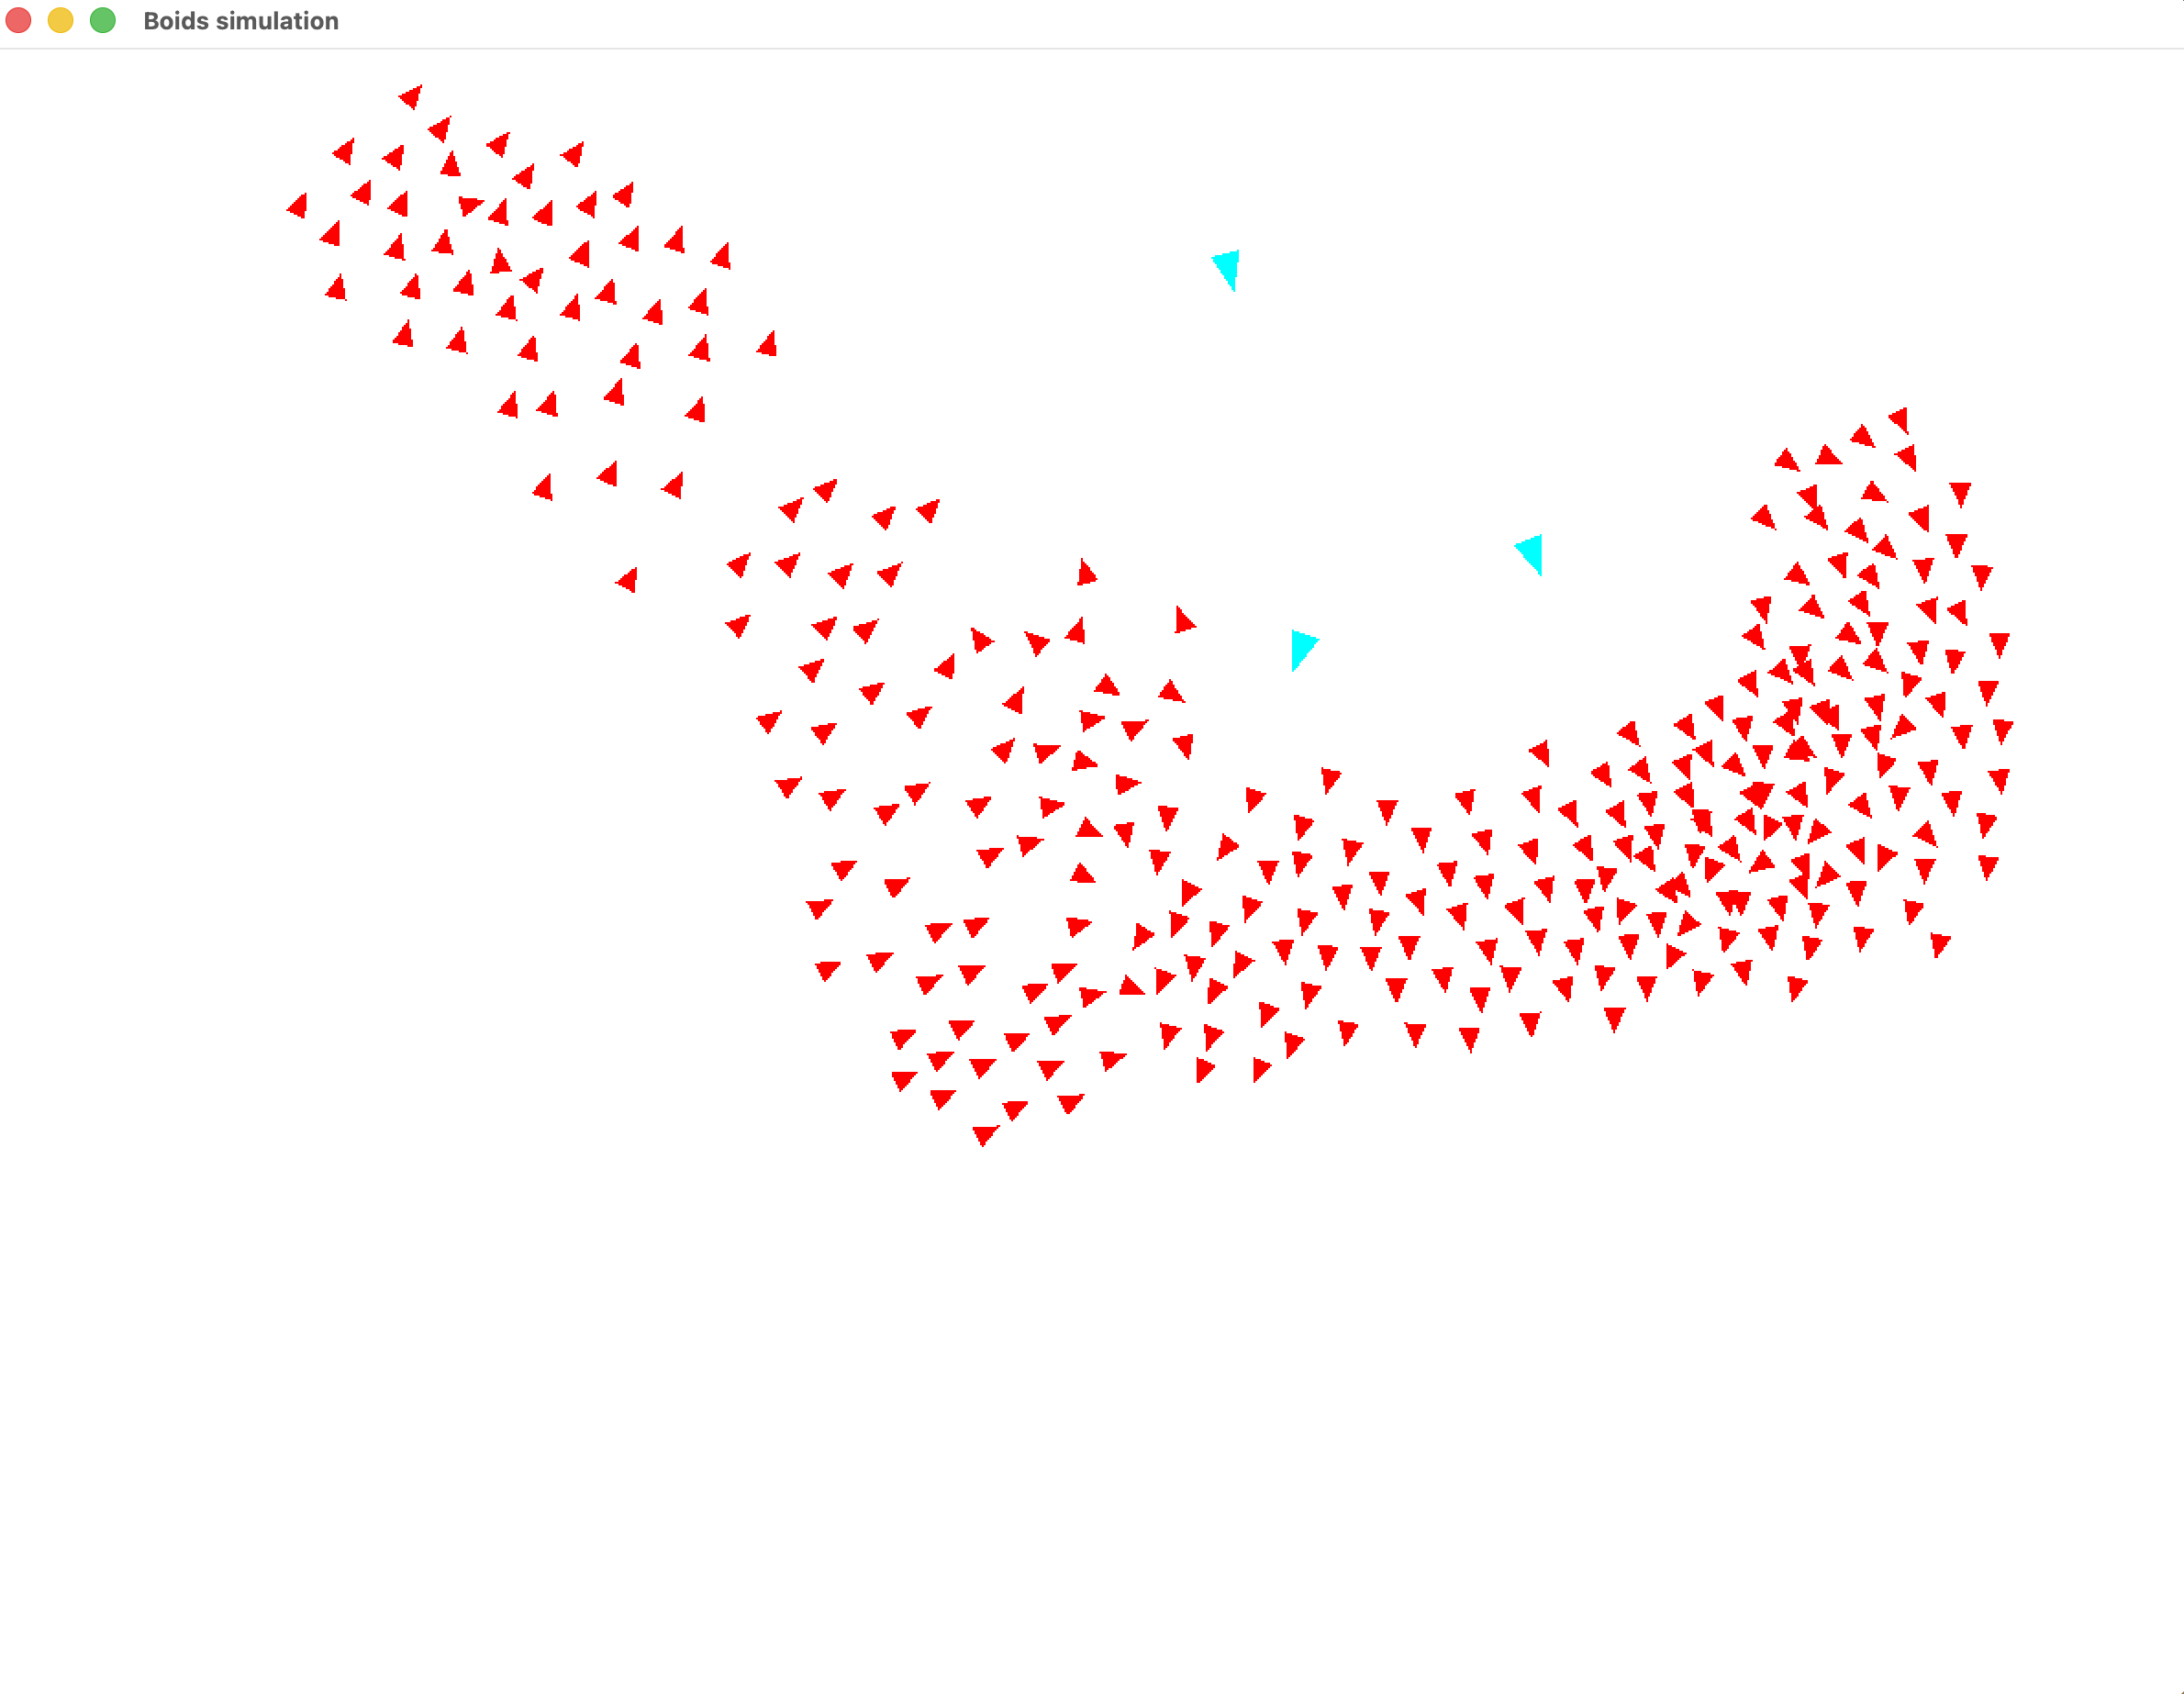
\includegraphics[width=\textwidth]{images/flock.png}
        \caption{} 
        \label{subfig:a}
    \end{subfigure}
    \begin{subfigure}[b]{0.45\textwidth}
        \centering
        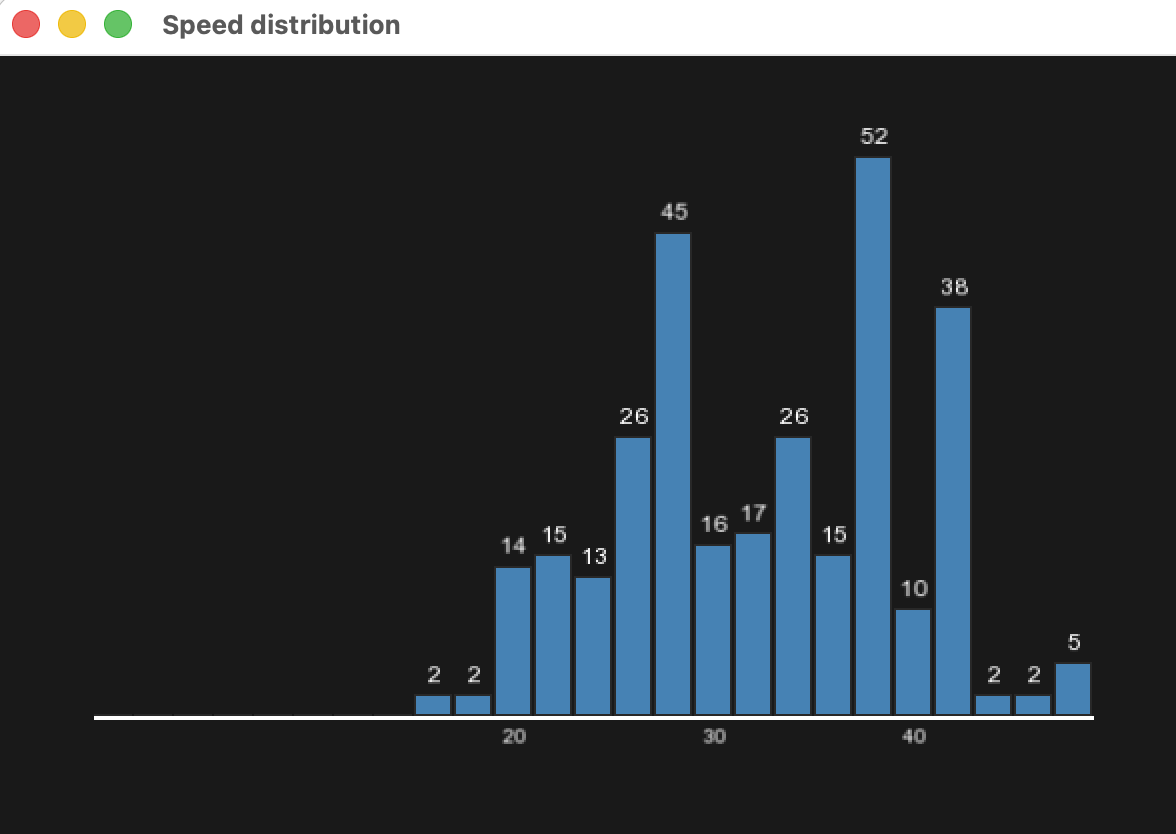
\includegraphics[width=\textwidth]{images/stats.png}
        \caption{}
        \label{subfig:b}
    \end{subfigure}
    \hfill
    \caption{Simulazione di uno stormo mediante il modello di Reynolds: in figura (a) in rosso sono rappresentati i \texttt{boids} mentre in azzurro sono disegnati gli \texttt{hunters}, in (b) la finestra mostra la distribuzione delle velocità dei \texttt{boids}.}
    \label{fig:boids}
\end{figure}
\section{Dichiarazione sull'uso di IA Generativa}
\label{sec:ia}
In accordo con i vincoli di trasparenza del corso, si dichiara che il modello di Intelligenza Artificiale Generativa Gemini è stato utilizzato esclusivamente come supporto per lo studio delle funzioni della libreria SFML (la quale esulava dal programma approfondito a lezione), per la ricerca di algoritmi e l'interpretazione di messaggi di errore del compilatore. La progettazione logica finale del sistema, l'implementazione software delle equazioni fisiche in C++, l'integrazione delle chiamate grafiche e il debugging finale rimangono interamente frutto dell'analisi e del lavoro originale del gruppo.

\end{document}